%!TEX root = ../template.tex
%%%%%%%%%%%%%%%%%%%%%%%%%%%%%%%%%%%%%%%%%%%%%%%%%%%%%%%%%%%%%%%%%%%%
%% chapter3.tex
%% NOVA thesis document file
%%
%% Chapter with a short latex tutorial and examples
%%%%%%%%%%%%%%%%%%%%%%%%%%%%%%%%%%%%%%%%%%%%%%%%%%%%%%%%%%%%%%%%%%%%

\typeout{NT FILE chapter3.tex}%

\chapter{Results}
\label{cha:results}

% Added introduction to the Results section
The Results section presents the aggregated data from the conducted experiments. Table \ref{tab:results} summarizes the key metrics evaluated for each question ID. 

       {\small
        \bgroup
\rowcolors{1}{}{GhostWhite}
\begin{xltabular}{\textwidth}{ccccccc}
    \caption{Test results summary.}
    \label{tab:results}\\
    \toprule
    \rowcolor{Gainsboro}%
    \textbf{\shortstack{Question \\ ID}} & \textbf{\shortstack{Completion \\ Rate}} & \textbf{\shortstack{Macro \\ Precision}} & \textbf{\shortstack{Macro \\ recall}} & \textbf{\shortstack{Macro \\ Soft F1-score}} & \textbf{\shortstack{Frequency \\ of the mode}} & \textbf{\shortstack{Consistency \\ Entropy}} \\
    \midrule
    \hyperref[question:1]{Question 1} & 100\% & 0.9988 & 0.9988 & 0.9988 & 1.0000 & 1.0000 \\
    \hyperref[question:2]{Question 2} & 100\% & 0.9667 & 0.8722 & 0.8772 & 0.9000 & 0.5310 \\
    \hyperref[question:3]{Question 3} & 90\% & 0.8831 & 0.7537 & 0.7680 & 0.5556 & 0.1472 \\
    \hyperref[question:4]{Question 4} & 100\% & 0.9630 & 0.9630 & 0.9630 & 1.0000 & 1.0000 \\
    \hyperref[question:5]{Question 5} & 100\% & 0.9316 & 0.9165 & 0.9187 & 0.9000 & 0.5310 \\
    \hyperref[question:6]{Question 6} & 100\% & 0.9672 & 0.9081 & 0.9367 & 1.0000 & 1.0000 \\
    \hyperref[question:7]{Question 7} & 100\% & 0.9988 & 0.9988 & 0.9988 & 1.0000 & 1.0000 \\
    \hyperref[question:8]{Question 8} & 100\% & 0.7737 & 1.0000 & 0.8516 & 0.5000 & 0.0628 \\
    \hyperref[question:9]{Question 9} & 100\% & 0.8202 & 0.9907 & 0.8858 & 0.4000 & 0.1390 \\
    \hyperref[question:10]{Question 10} & 100\% & 0.9588 & 0.9988 & 0.9738 & 0.9000 & 0.5310 \\

    \bottomrule
    \end{xltabular}
\egroup
}

\begin{figure}[htbp]
    \centering
    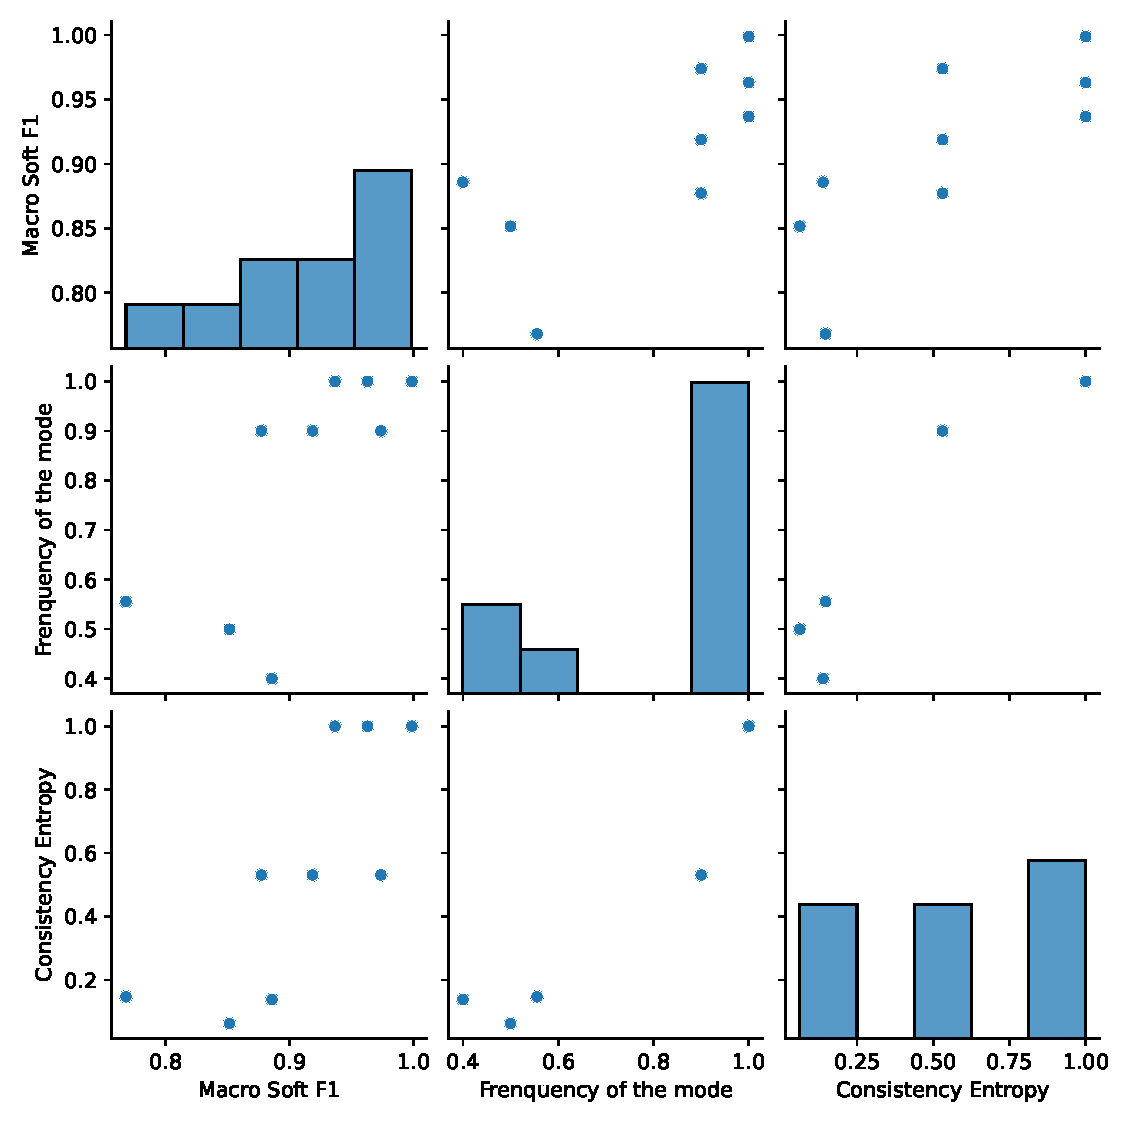
\includegraphics[width=\textwidth]{metrics_scattermatrix}
    \caption{Scatter matrix of evaluation metrics. Each point represents a question.}
    \label{fig:metrics_scattermatrix}
\end{figure}

TODO add figures selected 2 good and 2 bad maps


% Added interpretation of the results
The table highlights that most question IDs maintain a high completion rate and macro F1 scores, indicating consistent performance. Notably, Question ID 3 exhibits a lower completion rate and macro recall, suggesting areas for improvement in that category. 

The completion rate for most questions is 100\%, indicating that the system successfully generated and executed SQL queries without errors. However, Question ID 3 has a completion rate of 90%, suggesting that the system occasionally struggles with interpreting or executing queries related to single-family or two-family homes.

\section{Macro Precision, Recall, and Soft F1-Score}
The macro precision and recall metrics provide insights into the system's accuracy in retrieving relevant data. High precision indicates that the system retrieves relevant data points accurately, while high recall shows that it captures most of the relevant data. The Soft F1-score balances these two metrics, providing a comprehensive measure of performance. Questions 1 and 7 exhibit the highest F1 scores (> 0.99), demonstrating the system's strong performance in these areas. Conversely, Questions 2, 3, 8, and 9 have lower F1 scores (< 0.90), indicating potential areas for improvement.

\section{Consistency Metrics}
Consistency Entropy and Frequency of the Mode are used to assess the stability of the system's outputs. Lower entropy values indicate higher consistency, while a high mode frequency suggests that the system consistently produces the same output for repeated queries. Most questions show high consistency, with entropy values close to zero and mode frequencies near 1.0. However, Question 3 has a higher entropy value, reflecting variability in the system's outputs for this query.


\section{Interpretation of Specific Results}
The results for Question ID 3 highlight a need for further refinement in handling queries related to single-family or two-family homes. The lower completion rate and higher entropy suggest that the system may benefit from additional training or adjustments to better interpret and execute these specific queries.

Overall, the results demonstrate the system's robustness and reliability in generating accurate and consistent SQL queries for most evaluation questions. The identified areas for improvement provide valuable insights for future development and optimization efforts.

% \begin{newpdflayout}{210mm}{297mm}%{420mm}
% \end{newpdflayout}
